% ----- Fonctionnement -----

\subsection{How it works}

    To explain how our algorithm works, we will keeps track of two groups of vertices : $S$ which is a partially constructed (non-maximal) clique and the partial solution that we will gradually implement. Moreover, we got $P$  which is the candidates vertices that could be included in the clique, and which represents the union of all vertex neighbors of the vertices in $S$. Furthermore, we got $W$ which is the total weight of $S$ that we will implement
    \\ \\
    The algorithm begins by identifying the vertex with the highest sum of weights of its edges. If there are multiple vertices with the same maximum sum, the vertex with the highest degree is selected. The selected vertex is then added to $S$ and its neighbors are added to $P$. Then the algorithm selects a new vertex from the candidates set $P$ and adds it to $S$. We add to $W$ the weight of the edge between the new vertex selected and every vertices in $S$. This selected vertex is the one with the most weighted edge among all the vertices in $P$. After this step, $P$ is updated by considering only the neighbors of the vertices that are already part of $S$, and by excluding the vertices that are already part of $S$ from $P$. This process is then repeated until no more vertices are left in $P$, at which point the algorithm has obtained its maximum clique $S$.
    \\ \\
    To illustrate the Constructive algorithm, let's use the example in
    Figure \ref{fig:basic-graph-example} on page \pageref{fig:basic-graph-example} while adding some weight to its edges: \\

    \begin{minipage}{\linewidth}
        \textbf{Step 0:} \newline
        \begin{minipage}{0.4\textwidth}
            \begin{figure}[H]
                \centering
                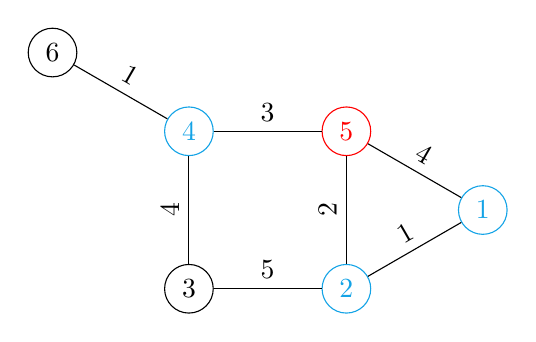
\begin{tikzpicture}[node distance=2cm]
                    \node[circle, draw, Cerulean] (1) {1};
                    \node[circle, draw, Cerulean] (2) at ([shift=(210:2)] 1) {2};
                    \node[circle, draw] (3) [left of=2] {3};
                    \node[circle, draw, Cerulean] (4) [above of=3] {4};
                    \node[circle, draw, red] (5) [above of=2] {5};
                    \node[circle, draw] (6) at ([shift=(150:2)] 4) {6};
    
                    \draw  (1) -- (2) node[midway, above, sloped] {1};
                    \draw (1) -- (5) node[midway, above, sloped] {4};
                    \draw (2) -- (3) node[midway, above, sloped] {5};
                    \draw (2) -- (5) node[midway, above, sloped] {2};
                    \draw (3) -- (4) node[midway, above, sloped] {4};
                    \draw (4) -- (5) node[midway, above, sloped] {3};
                    \draw (4) -- (6) node[midway, above, sloped] {1};
                \end{tikzpicture}
                \caption{Graph illustration for the constructive algorithm at step 0}
                \label{fig:constructive-mewc-edge}
            \end{figure}
        \end{minipage}
        \begin{minipage}{0.6\textwidth}
            At the initial step, as said before, we will initialize $S$ and $P$ by searching for the vertex with highest sum of weights of its edges $v$ by iterating every vertex on the graph. In this example, we will eventually find 3 and 5 which have a maximum sum of 9. The algorithm will then take the vertex of highest degree between them represented in \textcolor{red}{red} and will add it to $S$. The neighboring vertex of $v$ represented in \textcolor{Cerulean}{blue} will be added to $P$.
    
            \begin{center}
                \begin{tabular}{|lll|}
                    \hline
                    S = \{5\} & P = \{1,2,4\} & W = 0 \\
                    \hline
                \end{tabular}
            \end{center}
        \end{minipage}
    \end{minipage} 
    
    \vspace{1\baselineskip}

    \begin{minipage}{\linewidth}
        \textbf{Step 1:} \newline
        \begin{minipage}{0.4\textwidth}
            \begin{figure}[H]
                \centering
                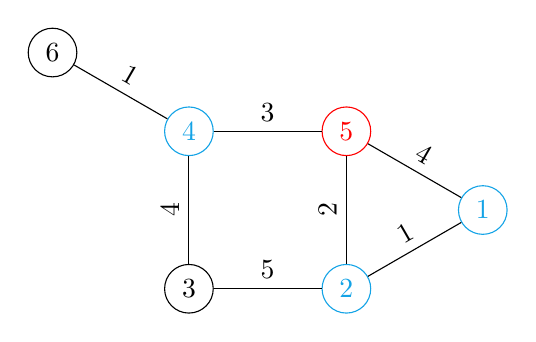
\begin{tikzpicture}[node distance=2cm]
                    \node[circle, draw, Cerulean] (1) {1};
                    \node[circle, draw, Cerulean] (2) at ([shift=(210:2)] 1) {2};
                    \node[circle, draw] (3) [left of=2] {3};
                    \node[circle, draw, Cerulean] (4) [above of=3] {4};
                    \node[circle, draw, red] (5) [above of=2] {5};
                    \node[circle, draw] (6) at ([shift=(150:2)] 4) {6};
    
                    \draw  (1) -- (2) node[midway, above, sloped] {1};
                    \draw (1) -- (5) node[midway, above, sloped] {4};
                    \draw (2) -- (3) node[midway, above, sloped] {5};
                    \draw (2) -- (5) node[midway, above, sloped] {2};
                    \draw (3) -- (4) node[midway, above, sloped] {4};
                    \draw (4) -- (5) node[midway, above, sloped] {3};
                    \draw (4) -- (6) node[midway, above, sloped] {1};
                \end{tikzpicture}
                \caption{Graph illustration for the constructive algorithm at step 0}
                \label{fig:constructive-mewc-edge}
            \end{figure}
        \end{minipage}
        \begin{minipage}{0.6\textwidth}
            
    
            \begin{center}
                \begin{tabular}{|ll|}
                    \hline
                    S = \{\} & P = \{1,2,4\} \\
                    \hline
                \end{tabular}
            \end{center}
        \end{minipage}
    \end{minipage} \newline
\newpage

